\documentclass[twoside, final, 11pt]{articleMine}
\usepackage[english]{babel} \usepackage{a4wide}
\usepackage{amsmath,amssymb,accents} \usepackage{epsfig}
\usepackage{subfigure} \usepackage{units} \usepackage{graphicx}
\usepackage[displaymath, mathlines, right]{lineno} \usepackage{xspace}
\usepackage{color} \usepackage{epic,eepic,pstricks}
\usepackage{acronym} \usepackage{wrapfig,multicol}
\usepackage{deluxetable} \usepackage{todonotes} 
\usepackage{hyperref}
\usepackage{float}
%\usepackage{slashbox}
\usepackage{lmodern} 
%\usepackage{caption}
\linenumbers
%\usepackage{showlabels}
\usepackage[draft]{showkeys}

%\usepackage[nolists, tablesfirst]{endfloat}
\graphicspath{{plots/}}
\newcommand*\patchAmsMathEnvironmentForLineno[1]{%
  \expandafter\let\csname old#1\expandafter\endcsname\csname #1\endcsname
  \expandafter\let\csname oldend#1\expandafter\endcsname\csname end#1\endcsname
  \renewenvironment{#1}%
     {\linenomath\csname old#1\endcsname}%
     {\csname oldend#1\endcsname\endlinenomath}}%
\newcommand*\patchBothAmsMathEnvironmentsForLineno[1]{%
  \patchAmsMathEnvironmentForLineno{#1}%
  \patchAmsMathEnvironmentForLineno{#1*}}%
\AtBeginDocument{%
\patchBothAmsMathEnvironmentsForLineno{equation}%
\patchBothAmsMathEnvironmentsForLineno{align}%
\patchBothAmsMathEnvironmentsForLineno{flalign}%
\patchBothAmsMathEnvironmentsForLineno{alignat}%
\patchBothAmsMathEnvironmentsForLineno{gather}%
\patchBothAmsMathEnvironmentsForLineno{multline}%
}
%\AtBeginFigures{\cleardoublepage}
%%%%%\parindent 5pt  
\parskip 1.2pt           % sets spacing between paragraphs
\def\Offline{\mbox{$\overline{\rm
Off}$\hspace{.05em}\raisebox{.4ex}{$\underline{\rm line}$}}\xspace}
\def\OfflineB{\mbox{$\bf\overline{\rm\bf
Off}$\hspace{.05em}\raisebox{.4ex}{$\bf\underline{\rm\bf line}$}}\xspace}

\def\eq#1{\begin{equation}#1\end{equation}}
%\def\al#1{\begin{align}#1\end{align}}
%\def\vc#1{{\bf #1}}
\def\pt#1{\accentset{\rightharpoonup}{#1}}
\include{myabbr}

\newcommand{\HRule}{\rule{\linewidth}{0.5mm}}
\newcommand{\VEM}{\mbox{VEM}}
\newcommand{\m}{\mbox{m}}

\let\stdsection\section  
%\renewcommand\section{\newpage\stdsection}  
 
\begin{document}

%\setpagewiselinenumbers
\modulolinenumbers[2]

%\linenumbers


\renewcommand\linenumberfont{\small\rmfamily}
\begin{center}
  \vspace*{-13ex}

  \rule{\linewidth}{0.1mm}  \\[17mm] {\huge  Matched filtering for EASIER data}
     \begin{flushright}
       \small 
     
     \end{flushright}

  % 
\end{center}
% 
\vspace*{2ex} 
%
\thispagestyle{empty}
\noindent
\begin{abstract}
  \noindent
We introduce in this note the method of matched filtering to EASIER data.
\end{abstract}

%
\thispagestyle{empty}
%$\;$
%\listoftodos
%\newpage
\noindent
\section{Introduction}
The  IPN software  is inherited  from  a Karlsruhe  software that  was
adapted by Francesco for EASIER  and then modified by Olivier and Imen
to introduce their way to compute  the MBR signal. We aim at giving an
overview of the functionning of the software here. \\ 


\section{Checks}
Here we compare the results we obtain with others. 
\subsection{Gorham shower}
Gorham shower, or the reference  shower is a vertical, \unit[$\rm 3.36
  \  10^{17}$]{eV}  shower,   observed  at  \unit[10]{km}.   The  flux
originally  calculated in~\cite{gorham} is  \unit[$\rm F_{ref}  = 2.77
  \ 10^{-24}$]{$\rm W.m^{-2}.Hz^{-1}$}.   \\ We simulate the reference
shower and record the flux at several distances. The results are given
in figure~\ref{refshower}.  We have set the units the same way than in
in~\cite{imen2016}.
\begin{figure}[ht!]
  \centering
  \hspace*{-3ex}
  \subfigure{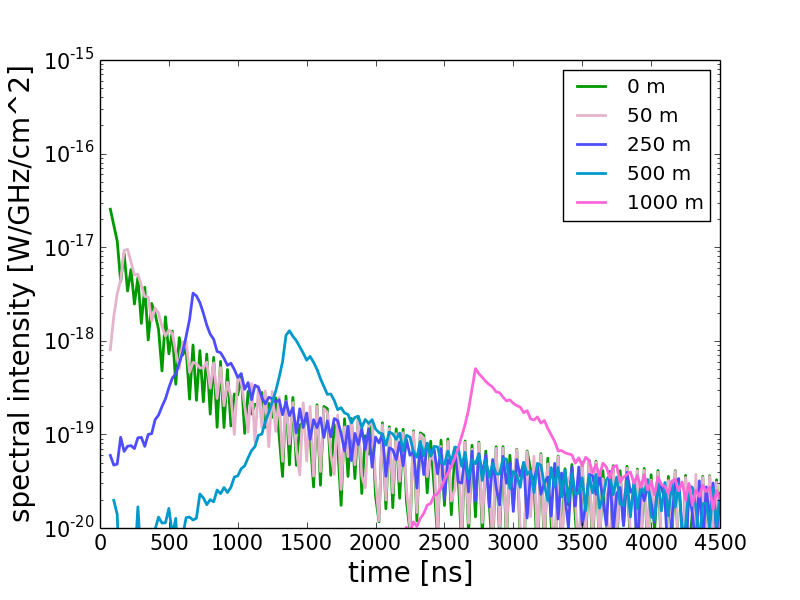
\includegraphics[width=0.49\linewidth]{myrefshower.png}}
  \subfigure{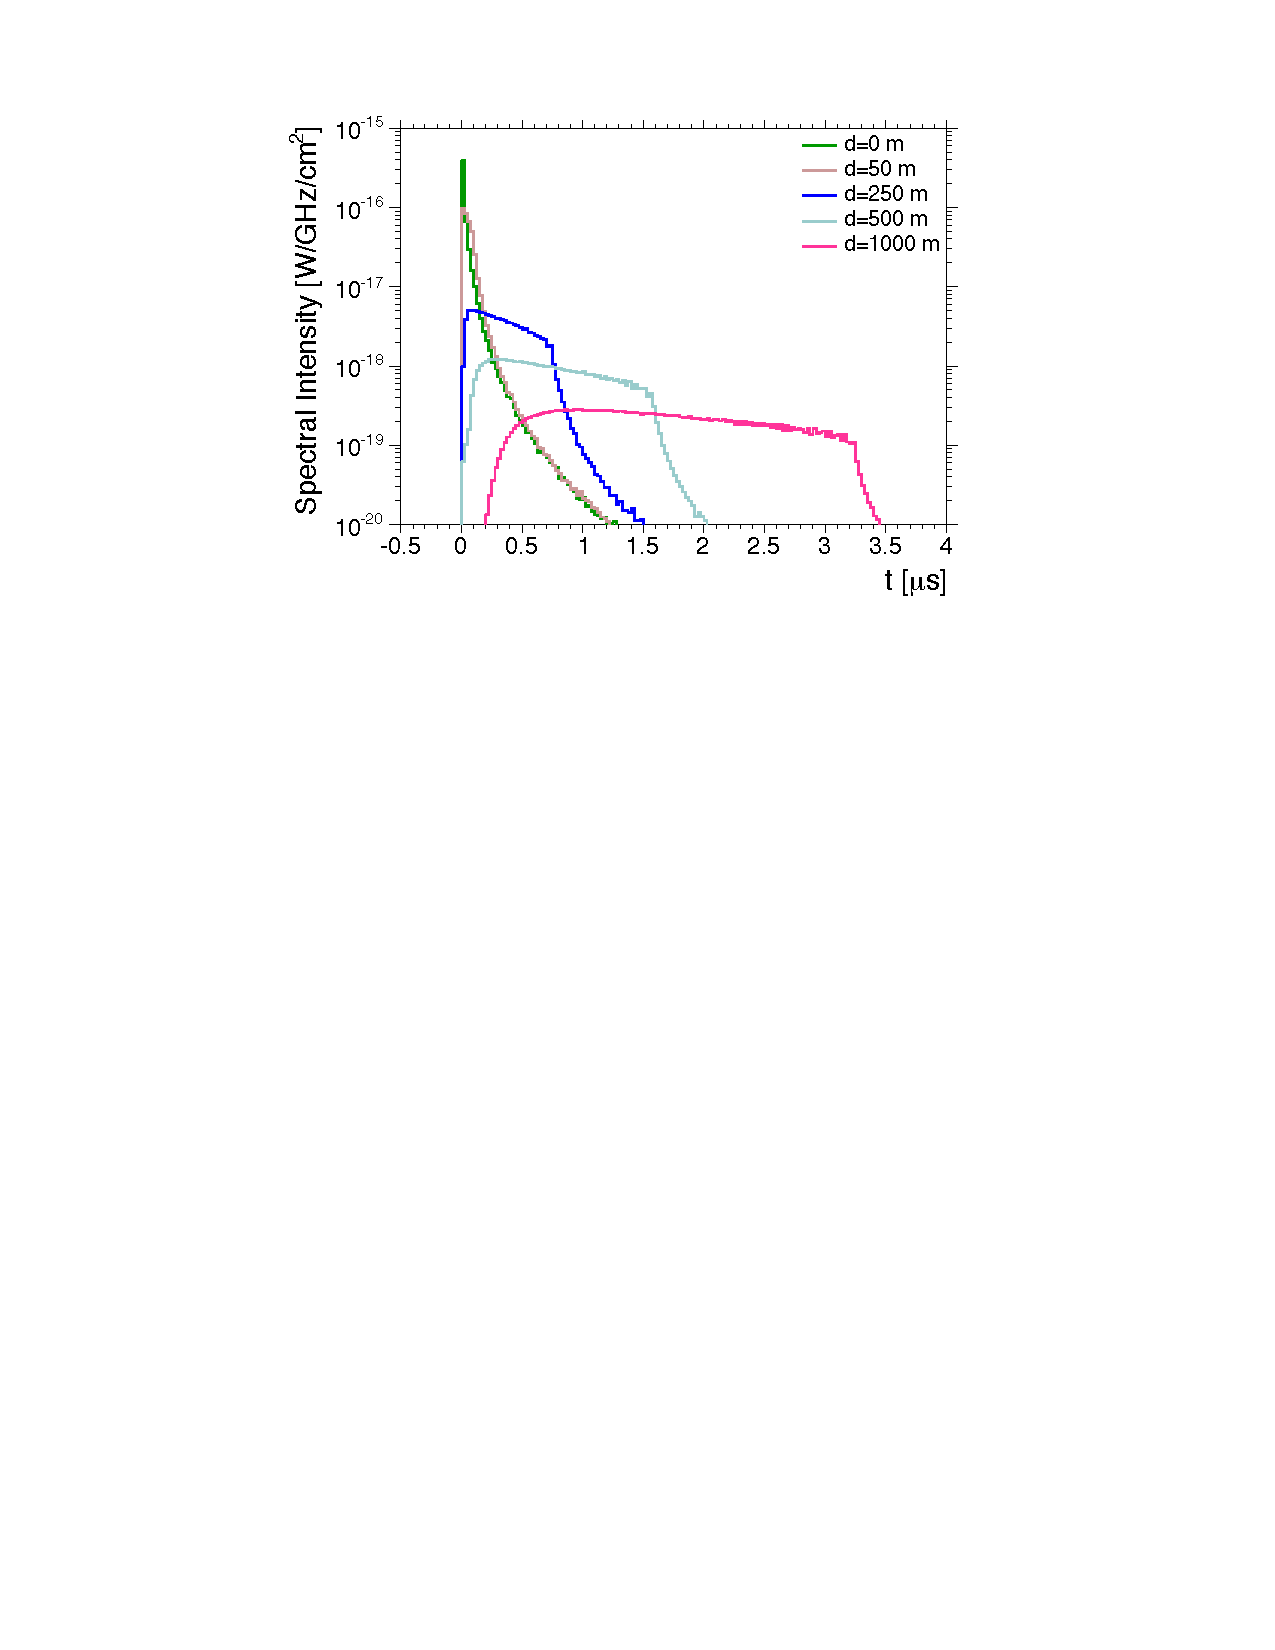
\includegraphics[width=0.49\linewidth]{paperrefshower.pdf}}
  \caption{three example of simulated trace with on top of each figure
    the signal in ADC counts, and on the bottom the signal in sigma}
  \label{fig:traceex}
\end{figure}

%%\section{Description}
lalalala

%%\include{conclusion/conclusion}

\addcontentsline{toc}{chapter}{Bibliography}                                 
\bibliographystyle{atlasnote}
\bibliography{thebib}
%% \newpage

\end{document}
